\begin{answer}{bivariatenormalmax}
Contrary to the above, there isn't always a pretty solution, sometimes we will have to do all the calculations.
This question is particularly nasty since it requires some niche definitions.
Doing the whole question isn't possible in the 10 minutes you will be allocated, so the interviewer is probably testing how well you perform under pressure,
how you approach a difficult problem by breaking it into smaller parts,
and what notation you use.

Get started in a direction, and try to think out loud:
``We want to evaluate an expectation, so we have to do an integral.''
Don't be afraid to ask the interviewer things like ``Do you think I'm on the right track?''
They will often offer little hints to help you along.
The last thing you want to do is get started on the wrong track and struggle with it for ten minutes while the interviewer sits there watching in silence.\footnote{During one of my interviews the interviewer started doing something on his phone while I was attempting the problem. No matter how I prodded, I couldn't get the guy interested in the interview. You win some, you lose some.}
Try to get the interviewer involved, but not to such an extent that it looks like you want them to hold your hand.
This is something that takes practise.
For our current problem, we have to write it into something easier first,
\[
  \max(X, Y) =
  \begin{dcases*}
    Y & if $Y \geq X$\\
    X & if $X < Y$
  \text{.}
  \end{dcases*}
\]
Now we can use the Law of Total Expectation:
\index{Tricks!Law of Total Expectation}
If $ A_1, A_2, A_3, \ldots, A_n$ are mutually disjoint and exhaustive, then
\[
  \E(Z) = \sum_{i=1}^{n}{
    \E(Z| A_i)P(A_i)
  }
  \text{.}
\]
You've probably never had to use it in this form before, but it comes in handy for this brainteaser.
In our case, let $Z=\max(X,Y)$, with the expectation expanded as
\begin{align*}
  \E(Z) &= \E(Z|X > Y)P(X>Y)
+          \E(Z|X \leq Y)P(X \leq Y) \\
        &= \E(X|X > Y)P(X>Y)
+          \E(Y|X \leq Y)P(X \leq Y)
  \text{.}
\end{align*}
Now the interviewer will point out that the two terms on the right-hand side are symmetric, thus they must be the same:
\[
  \E(Z) = 2 \E(X|X > Y)P(X>Y)
  \text{.}
\]
Here, $P(X>Y) = \nicefrac{1}{2}$ and doesn't depend on $\rho$.
The integration that proves this is tedious and again it is easier to draw a picture; below is a contour plot of the bivariate normal distribution with
\[
\vec{\mu}=
\begin{bmatrix}
  0    \\
  0
\end{bmatrix}
\text{ and }
\Sigma =
\begin{bmatrix}
  1    & \rho \\
  \rho & 1    \\
\end{bmatrix}
\]
for different values of $\rho$.
The contour plot is something you can quickly draw by hand in an interview.
The three-dimensional plot that appears under it is not, but it is included for clarity.
\begin{center}
  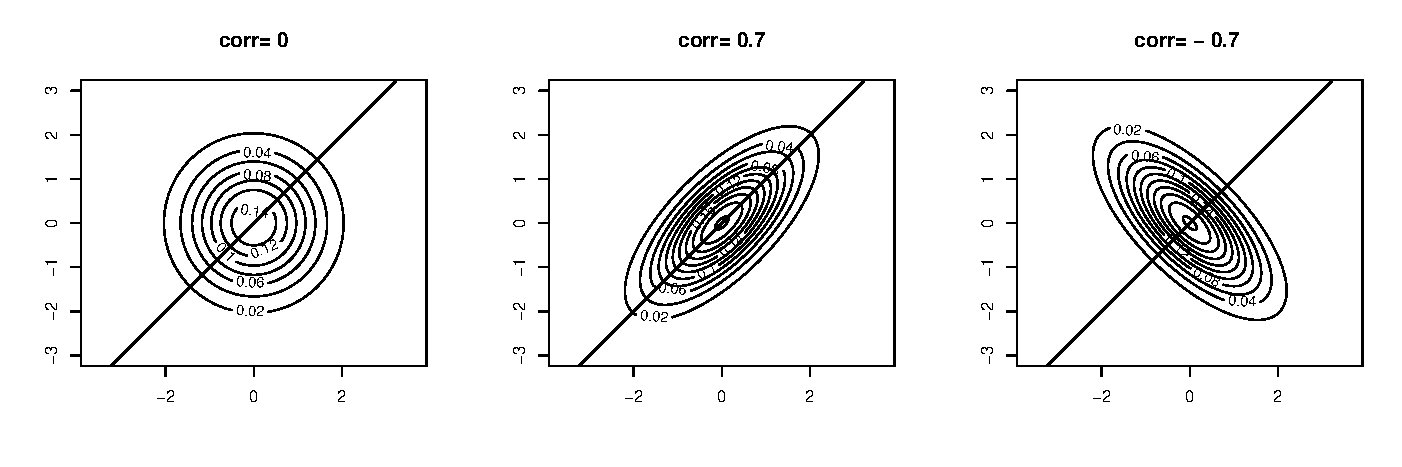
\includegraphics[width=\textwidth]{./plots/mvtnorm/mvrnorm.pdf}
  % mvrnorm.pdf: 0x0 pixel, 300dpi, 0.00x0.00 cm, bb=
  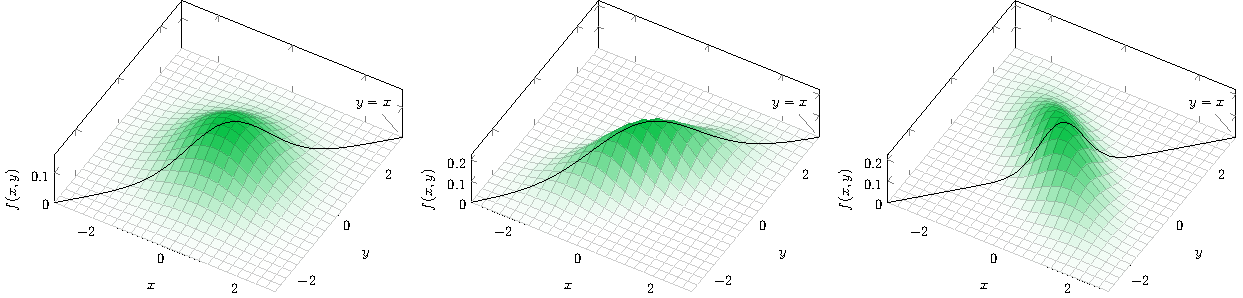
\includegraphics[width=\textwidth]{./plots/bivariatenorm/bivariatenorm.pdf}
\end{center}
The line shows $y=x$, and it is not hard to see that the area under the distribution where $x>y$ will be equal to \nicefrac{1}{2} for any value of $\rho$.
Thus we have reduced the problem to
\[
\E(Z) =  \E(X|X > Y)
\]
and we just need to find a smart way to evaluate it.
If you have gotten this far, the interviewer will probably be convinced of your ability to solve the problem and (hopefully) end it here and move on to the next question.
Some firms  ask really difficult questions, but they don't expect you to get the correct answer.
(This is especially the case with Goldman Sachs.)
They want to see how you think.
At some hedge funds I saw the opposite: They ask moderately difficult questions and snidely remark that you seem unable to do the ``simple proof'' which is quite trivial to them (especially after checking the solution just before the interview) if you don't start off on the right track immediately.
You win some, you lose some.

I will give the rest of the answer here for the sake of completeness, and then I will present a smart solution that a friend of mine provided.
You will notice that the solution is complicated and requires a fair amount of textbook theory, like the properties of a truncated normal distribution.
Even if you are able to recall all the required properties during an interview, doing a rigorous proof will take longer than the time allocated.
Again, the interviewer probably isn't looking for the whole proof, but rather the steps you would take during it.

The quantity $\E(X|X > Y)$ isn't immediately recognisable.
However, if we write it as
\begin{align*}
\E(X|X-Y > 0) = \E(W_1|W_2 > 0)
\end{align*}
it becomes a conditional expectation of two random variables that are a linear combination of our original bivariate normal distribution.
To see this, let
\[B =
\begin{bmatrix}
  1   &  0 \\
  1   & -1 \\
  \end{bmatrix}
\]
then
\[
\begin{bmatrix}
  W_1 \\ W_2
\end{bmatrix}
=
B
  \begin{bmatrix}
  X \\ Y
  \end{bmatrix}
  =
  \begin{bmatrix}
  X \\ X-Y
  \end{bmatrix}
  \text{.}
\]
This is an affine transformation of a multivariate normal distribution, which is also multivariate normal:
\[
\begin{bmatrix}
  W_1 \\ W_2
\end{bmatrix}
=
B
\begin{bmatrix}
X \\ Y
\end{bmatrix}
\sim
\operatorname{MultivariateNormal}
\left(
B
\begin{bmatrix}
0 \\ 0
\end{bmatrix}
  ,
  B
  \begin{bmatrix}
  1      &   \rho \\
  \rho   &   1    \\
  \end{bmatrix}
  B^T
  \right)
  \text{.}
\]
Thus
\[
\begin{bmatrix}
W_1 \\ W_2
\end{bmatrix}
=
\begin{bmatrix}
X \\ X - Y
\end{bmatrix}
\sim
\operatorname{MultivariateNormal}
\left(
\begin{bmatrix}
0 \\ 0
\end{bmatrix}
,
\begin{bmatrix}
        1 &    1 -\rho \\
  1-\rho  &  2(1 - \rho)
\end{bmatrix}
  \right)
\]
and we can use the conditional properties of the multivariate normal distribution to evaluate
\begin{equation}
\label{eq:bivariatenormalmax:conditional_expecation}
\E(X|X-Y > 0)
\end{equation}
as
\begin{equation*}
\E(W_1|W_2 > 0)
\text{.}
\end{equation*}
This conditional expectation is difficult to evaluate.
If we partition
\[
\vec{x} \sim \operatorname{MultivariateNormal}(\vec{\mu}, \vec{\Sigma})
\]
into
\[
\begin{bmatrix}
\vec{x}_1 \\ \vec{x}_2
\end{bmatrix}
\sim
\operatorname{MultivariateNormal}
\left(
\begin{bmatrix}
\vec{\mu}_1 \\ \vec{\mu}_2
\end{bmatrix}
,
\begin{bmatrix}
\vec{\Sigma}_{11} & \vec{\Sigma}_{12} \\
\vec{\Sigma}_{21} & \vec{\Sigma}_{22} \\
\end{bmatrix}
  \right)
\]
we know from the theory of the multivariate normal distribution that
\[
  (\vec{x}_1 | \vec{x}_2 =  \vec{a})
  \sim
\operatorname{MultivariateNormal}
\left(
\vec{\mu}_1 +
\vec{\Sigma}_{12}
\vec{\Sigma}_{22}^{-1}
(\vec{a} - \vec{\mu}_2)
\, , \,
\vec{\Sigma}_{11}
-
\vec{\Sigma}_{12}
\vec{\Sigma}_{22}^{-1}
\vec{\Sigma}_{21}
  \right)
\text{.}
\]
In our example, this means
\begin{align*}
\E(W_1|W_2 = w_2) &=  \frac{(1-\rho)}{2(1-\rho)} w_2 \\
                  &=  \frac{1}{2}w_2
\text{.}
\end{align*}
Using (somewhat liberally) the tower property of the Law of Total Expectation,
\begin{align*}
\E(X \, | \, f(Y)) &=
\E( \E(X\,|\,Y) \; | \; f(Y))
\text{,}
\end{align*}
we can write
\begin{align*}
\E(W_1|W_2 > 0 )
&=
\E( \E(  W_1| W_2) \;|\; W_2 > 0 ) \\
&= \E\left( \frac{1}{2}W_2 \; \Bigg| \; W_2>0 \right) \\
&= \frac{1}{2}\E( W_2 | W_2>0 )
\text{.}
\end{align*}
This is $\nicefrac{1}{2}$ multiplied by the expected value of a truncated normal distribution,
\begin{align}
\E(W_2|W_2 > 0)
&= 0 + \frac{ \sqrt{2( 1- \rho)} \phi(0)}{1- \Phi(0)} \label{eq:bivariatenormalmax:conditional_expecation2} \\
&=  \frac{ \sqrt{2( 1- \rho)} \frac{1}{\sqrt{2 \pi}} }{\frac{1}{2}} \nonumber \\
&=  \frac{ 2 \sqrt{ 1- \rho}  }{ \sqrt{ \pi} } \nonumber
\text{.}
\end{align}
Putting it all together we finally arrive at the answer.
\begin{align*}
\E(Z) &=  \E(X|X > Y)  \\
      &= \E(W_1|W_2 > 0 ) \\
      &= \frac{1}{2}E(W_2|W_2>0) \\
      &=  \frac{1}{2}\frac{ 2 \sqrt{ 1- \rho}  }{ \sqrt{ \pi} } \\
      &=  \sqrt{\frac{ 1- \rho  }{ \pi }}
\text{.}
\end{align*}
You can use Monte Carlo integration to convince yourself of this; I include an R script in appendix \ref{ap:mvtnormproof} to do just that.




The solution provided by my friend starts out different.
It uses the identity
\[
  \max(x,y) = \frac{x + y + |x-y|}{2}
\]
which we can also refer to as a trick.
Using this, the expectation becomes
\begin{align*}
  \E(\max(X,Y))
  &= \frac{1}{2}\E(X + Y + |X-Y|) \\
  &= \frac{1}{2}\E(|X-Y|) \qquad \text{because } \E(X) = \E(Y) = 0 \\
  &= \frac{1}{2}
  \bigg(
     \E(X-Y |X-Y > 0 ) P(X-Y > 0)  \\
  &\qquad + \E(Y-X |X-Y \leq 0 ) P(X-Y \leq 0)
  \bigg) \quad \text{total expectation} \\
  &= \frac{1}{2} 2
    \bigg(
      \E(X-Y |X-Y > 0 ) P(X-Y > 0)
    \bigg) \quad \text{symmetry} \\
  &=
    \E(X-Y |X-Y > 0 ) \frac{1}{2}
\text{.}
\end{align*}
The random variable $W_2 = X-Y$ has a $\text{Normal}(0, 2(1-\rho))$ distribution.
To see this, use a matrix $B=
\begin{bmatrix}
        1 &    -1 \\
\end{bmatrix}
$ for an affine transformation as before, or consider that the sum of two random variables each from a normal distribution is itself a normal distribution, where you have to find
$\E(W_2) = \E(X-Y)$
and
$\Var(W_2) = \Var(X-Y)$.
So now we have
\begin{align*}
\E(X-Y|X-Y > 0) &=  \E(W_2|W_2 > 0)
\end{align*}
which is the same expectation we had in (\ref{eq:bivariatenormalmax:conditional_expecation2}), thus
\begin{align*}
\E(X-Y|X-Y > 0) =
 \frac{ 2 \sqrt{ 1- \rho}  }{ \sqrt{ \pi} }
\end{align*}
and
\[
\E(\max(X, Y)) = \sqrt{\frac{  1- \rho  }{  \pi }}
\text{,}
\]
corroborating our earlier answer.

\end{answer}

